\documentclass[journal,12pt,twocolumn]{IEEEtran}
\usepackage{setspace}
\usepackage{gensymb}
\usepackage{caption}
%\usepackage{multirow}
%\usepackage{multicolumn}
%\usepackage{subcaption}
%\doublespacing
\singlespacing
\usepackage{csvsimple}
\usepackage{amsmath}
\usepackage{multicol}
%\usepackage{enumerate}
\usepackage{amssymb}
%\usepackage{graphicx}
\usepackage{newfloat}
%\usepackage{syntax}
\usepackage{listings}
\usepackage{iithtlc}
\usepackage{color}
\usepackage{tikz}
\usetikzlibrary{shapes,arrows}



%\usepackage{graphicx}
%\usepackage{amssymb}
%\usepackage{relsize}
%\usepackage[cmex10]{amsmath}
%\usepackage{mathtools}
%\usepackage{amsthm}
%\interdisplaylinepenalty=2500
%\savesymbol{iint}
%\usepackage{txfonts}
%\restoresymbol{TXF}{iint}
%\usepackage{wasysym}
\usepackage{amsthm}
\usepackage{mathrsfs}
\usepackage{txfonts}
\usepackage{stfloats}
\usepackage{cite}
\usepackage{cases}
\usepackage{mathtools}
\usepackage{caption}
\usepackage{enumerate}	
\usepackage{enumitem}
\usepackage{amsmath}
%\usepackage{xtab}
\usepackage{longtable}
\usepackage{multirow}
%\usepackage{algorithm}
%\usepackage{algpseudocode}
\usepackage{enumitem}
\usepackage{mathtools}
\usepackage{hyperref}
%\usepackage[framemethod=tikz]{mdframed}
\usepackage{listings}
    %\usepackage[latin1]{inputenc}                                 %%
    \usepackage{color}                                            %%
    \usepackage{array}                                            %%
    \usepackage{longtable}                                        %%
    \usepackage{calc}                                             %%
    \usepackage{multirow}                                         %%
    \usepackage{hhline}                                           %%
    \usepackage{ifthen}                                           %%
  %optionally (for landscape tables embedded in another document): %%
    \usepackage{lscape}     


\usepackage{url}
\def\UrlBreaks{\do\/\do-}


%\usepackage{stmaryrd}


%\usepackage{wasysym}
%\newcounter{MYtempeqncnt}
\DeclareMathOperator*{\Res}{Res}
%\renewcommand{\baselinestretch}{2}
\renewcommand\thesection{\arabic{section}}
\renewcommand\thesubsection{\thesection.\arabic{subsection}}
\renewcommand\thesubsubsection{\thesubsection.\arabic{subsubsection}}

\renewcommand\thesectiondis{\arabic{section}}
\renewcommand\thesubsectiondis{\thesectiondis.\arabic{subsection}}
\renewcommand\thesubsubsectiondis{\thesubsectiondis.\arabic{subsubsection}}

% correct bad hyphenation here
\hyphenation{op-tical net-works semi-conduc-tor}

%\lstset{
%language=C,
%frame=single, 
%breaklines=true
%}

%\lstset{
	%%basicstyle=\small\ttfamily\bfseries,
	%%numberstyle=\small\ttfamily,
	%language=Octave,
	%backgroundcolor=\color{white},
	%%frame=single,
	%%keywordstyle=\bfseries,
	%%breaklines=true,
	%%showstringspaces=false,
	%%xleftmargin=-10mm,
	%%aboveskip=-1mm,
	%%belowskip=0mm
%}

%\surroundwithmdframed[width=\columnwidth]{lstlisting}
\def\inputGnumericTable{}                                 %%
\lstset{
%language=C,
frame=single, 
breaklines=true,
columns=fullflexible
}
 

\begin{document}
%
\tikzstyle{block} = [rectangle, draw,
    text width=3em, text centered, minimum height=3em]
\tikzstyle{sum} = [draw, circle, node distance=3cm]
\tikzstyle{input} = [coordinate]
\tikzstyle{output} = [coordinate]
\tikzstyle{pinstyle} = [pin edge={to-,thin,black}]

\theoremstyle{definition}
\newtheorem{theorem}{Theorem}[section]
\newtheorem{problem}{Problem}
\newtheorem{proposition}{Proposition}[section]
\newtheorem{lemma}{Lemma}[section]
\newtheorem{corollary}[theorem]{Corollary}
\newtheorem{example}{Example}[section]
\newtheorem{definition}{Definition}[section]
%\newtheorem{algorithm}{Algorithm}[section]
%\newtheorem{cor}{Corollary}
\newcommand{\BEQA}{\begin{eqnarray}}
\newcommand{\EEQA}{\end{eqnarray}}
\newcommand{\define}{\stackrel{\triangle}{=}}

\bibliographystyle{IEEEtran}
%\bibliographystyle{ieeetr}

\providecommand{\nCr}[2]{\,^{#1}C_{#2}} % nCr
\providecommand{\nPr}[2]{\,^{#1}P_{#2}} % nPr
\providecommand{\mbf}{\mathbf}
\providecommand{\pr}[1]{\ensuremath{\Pr\left(#1\right)}}
\providecommand{\qfunc}[1]{\ensuremath{Q\left(#1\right)}}
\providecommand{\sbrak}[1]{\ensuremath{{}\left[#1\right]}}
\providecommand{\lsbrak}[1]{\ensuremath{{}\left[#1\right.}}
\providecommand{\rsbrak}[1]{\ensuremath{{}\left.#1\right]}}
\providecommand{\brak}[1]{\ensuremath{\left(#1\right)}}
\providecommand{\lbrak}[1]{\ensuremath{\left(#1\right.}}
\providecommand{\rbrak}[1]{\ensuremath{\left.#1\right)}}
\providecommand{\cbrak}[1]{\ensuremath{\left\{#1\right\}}}
\providecommand{\lcbrak}[1]{\ensuremath{\left\{#1\right.}}
\providecommand{\rcbrak}[1]{\ensuremath{\left.#1\right\}}}
\theoremstyle{remark}
\newtheorem{rem}{Remark}
\newcommand{\sgn}{\mathop{\mathrm{sgn}}}
\providecommand{\abs}[1]{\left\vert#1\right\vert}
\providecommand{\res}[1]{\Res\displaylimits_{#1}} 
\providecommand{\norm}[1]{\left\Vert#1\right\Vert}
\providecommand{\mtx}[1]{\mathbf{#1}}
\providecommand{\mean}[1]{E\left[ #1 \right]}
\providecommand{\fourier}{\overset{\mathcal{F}}{ \rightleftharpoons}}
%\providecommand{\hilbert}{\overset{\mathcal{H}}{ \rightleftharpoons}}
\providecommand{\system}{\overset{\mathcal{H}}{ \longleftrightarrow}}
	%\newcommand{\solution}[2]{\textbf{Solution:}{#1}}
\newcommand{\solution}{\noindent \textbf{Solution: }}
\newcommand{\myvec}[1]{\ensuremath{\begin{pmatrix}#1\end{pmatrix}}}
\providecommand{\dec}[2]{\ensuremath{\overset{#1}{\underset{#2}{\gtrless}}}}
\DeclarePairedDelimiter{\ceil}{\lceil}{\rceil}
%\numberwithin{equation}{section}
%\numberwithin{problem}{subsection}
%\numberwithin{definition}{subsection}
\makeatletter
\@addtoreset{figure}{section}
\makeatother

\let\StandardTheFigure\thefigure
%\renewcommand{\thefigure}{\theproblem.\arabic{figure}}
\renewcommand{\thefigure}{\thesection}


%\numberwithin{figure}{subsection}

%\numberwithin{equation}{subsection}
%\numberwithin{equation}{section}
%\numberwithin{equation}{problem}
%\numberwithin{problem}{subsection}
\numberwithin{problem}{section}
%%\numberwithin{definition}{subsection}
%\makeatletter
%\@addtoreset{figure}{problem}
%\makeatother
\makeatletter
\@addtoreset{table}{section}
\makeatother

\let\StandardTheFigure\thefigure
\let\StandardTheTable\thetable
\let\vec\mathbf
%%\renewcommand{\thefigure}{\theproblem.\arabic{figure}}
%\renewcommand{\thefigure}{\theproblem}

%%\numberwithin{figure}{section}

%%\numberwithin{figure}{subsection}



\def\putbox#1#2#3{\makebox[0in][l]{\makebox[#1][l]{}\raisebox{\baselineskip}[0in][0in]{\raisebox{#2}[0in][0in]{#3}}}}
     \def\rightbox#1{\makebox[0in][r]{#1}}
     \def\centbox#1{\makebox[0in]{#1}}
     \def\topbox#1{\raisebox{-\baselineskip}[0in][0in]{#1}}
     \def\midbox#1{\raisebox{-0.5\baselineskip}[0in][0in]{#1}}

\vspace{3cm}

\title{ 
	\logo{
The Circle
	}
}

\author{ G V V Sharma$^{*}$% <-this % stops a space
	\thanks{*The author is with the Department
		of Electrical Engineering, Indian Institute of Technology, Hyderabad
		502285 India e-mail:  gadepall@iith.ac.in. All content in this manual is released under GNU GPL.  Free and open source.}
	
}	

\maketitle

%\tableofcontents

\bigskip

\renewcommand{\thefigure}{\theenumi}
\renewcommand{\thetable}{\theenumi}


\begin{abstract}
	Solved problems from JEE mains papers related to 2D circles in coordinate geometry are 
available in this document.  These problems are solved using linear algebra/matrix analysis.
\end{abstract}
\begin{enumerate}[label=\arabic*]
\numberwithin{equation}{enumi}
\item A circle passes through the points $\vec{A}=\myvec{2 \\ 3}$ and $\vec{B} = \myvec{4 \\  5}$.  If its centre $\vec{O}$ lies on the 
line
\begin{equation}
\label{eq:circle_1}
\myvec{-1 & 4}\vec{x} - 3 =0
\end{equation}
%
find its radius.
\\
\solution Let 
\begin{align}
\vec{C}=\frac{\vec{A}+\vec{B}}{2}
\implies \vec{C}=\myvec{3 \\ 4}
\label{eq:circle_1_c}
\end{align}
The direction vector of $AB$ is 
\begin{align}
\label{eq:circle_1_m}
\vec{m} = \myvec{2 \\ 3}-\myvec{4 \\  5}
= \myvec{-2 \\ -2}
\end{align}
\begin{align}
\because OC &\perp AB,
\nonumber \\
OC: \vec{m}^T\brak{\vec{x}-\vec{C}}&=0
\nonumber \\
\implies \myvec{1 & 1}\vec{x} &= 7
\label{eq:circle_1_oc}
\end{align}
%
Thus, $\vec{O}$ is the intersection of \eqref{eq:circle_1}
and \eqref{eq:circle_1_oc} and is the solution of the matrix equation
\begin{align}
 \myvec{1 & 1 \\ -1 & 4}\vec{x} &= \myvec{7 \\ 3}
\label{eq:circle_1_matrix}
\end{align}
%
From the augmented matrix,
\begin{align}
 \myvec{1 & 1 &7\\ -1 & 4 & 3}&\leftrightarrow  \myvec{1 & 1 &7\\ 0 & 1 & 2}\leftrightarrow \myvec{1 & 0 & 5\\ 0 & 1 & 2} 
\nonumber \\
\implies \vec{O} &= \myvec{5 \\ 2}
\label{eq:circle_1_o}
\end{align}
%
Thus the radius of the circle 
\begin{align}
\label{eq:circle_1_r}
OA = \norm{\vec{O}-\vec{A}} = \sqrt{10}
\end{align}
\item If a circle $C_1$, whose radius is 3, touches externally the circle 
\begin{equation}
\label{eq:circle_2_c2}
C_2: \vec{x}^T\vec{x} + \myvec{2 & -4}\vec{x} = 4
\end{equation}
%
at the point $\vec{P}=\myvec{2\\2}$, then find the length of the intercept cut by this circle $C$ on the $x$-axis.
\\
\solution From \eqref{eq:circle_2_c2}, the centre of $C_2$ is 
\begin{align}
\label{eq:circle_2_o2}
\vec{O}_2 = \myvec{-1 \\ 2}
\end{align}
%
The radius of the circle is given by 
\begin{align}
\label{eq:circle_2_r2}
r_2^2-\vec{O}_2^T\vec{O}_2 = 4 \implies r_2 = 3
\end{align}
%
%The direction vector of $O_2P$ is 
%\begin{align}
%\label{eq:circle_2_r2}
%\vec{O}_2-\vec{P} = \myvec{-3 \\ 0}
%\end{align}
%
Since the radius of $C_1$ is $r_1=r_2=3$ and $\vec{O}_1, \vec{P}, \vec{O}_2$ are collinear, 
\begin{align}
\label{eq:circle_2_o1}
\frac{\vec{O}_1+\vec{O}_2}{2} &= \vec{P}
\nonumber \\
\implies \vec{O}_1 &= 2\vec{P}-\vec{O}_2
\nonumber \\
\implies \vec{O}_1 &= \myvec{5 \\ 2}
\end{align}
%
The intercepts of $C_1$ on the $x-$axis can be expressed as 
\begin{align}
\label{eq:circle_2_x}
\vec{x}=\lambda\vec{m}
\end{align}
%
where
\begin{align}
\label{eq:circle_2_m}
\vec{m}=\myvec{1 \\ 0}
\end{align}
Susbtituting in the equation for $C_1$,
\begin{align}
\norm{\lambda\vec{m}-\vec{O}_1}^2&=r_1^2
\end{align}
which can be expressed as
\begin{align}
\lambda^2\norm{\vec{m}}^2-2\lambda\vec{m}^T\vec{O}_1+ \norm{\vec{O}_1}^2-r_1^2&=0
\nonumber \\
\implies \lambda^2-10\lambda+ 20&=0
\end{align}
resulting in
\begin{align}
\lambda&=5\pm\sqrt{5}
\label{eq:circle_2_lam}
\end{align}
%
after substituting from \eqref{eq:circle_2_m} and \eqref{eq:circle_2_o1}.


\item A line drawn through the point 
\begin{equation}
\label{eq:circle_3_p}
\vec{P} = \myvec{4\\7} 
\end{equation}
cuts the circle
\begin{equation}
\label{eq:circle_3}
C: \vec{x}^T\vec{x}  = 9
\end{equation}
at the points $\vec{A}$ and $\vec{B}$. Find $PA.PB$. Draw $PAB$ for any two points $\vec{A},\vec{B}$ on the circle.
\\
\solution Since the points $\vec{P},\vec{A},\vec{B}$ are collinear, the line $PAB$ can be expressed as
\begin{align}
L: \vec{x} = \vec{P} + \lambda \vec{m}
\label{eq:circle_3_pab}
\end{align}
%
for $\norm{\vec{m}} = 1$. The intersection of $L$ and $C$  yields
\begin{align}
\brak{\vec{P}+ \lambda \vec{m}}^T
% }
\brak{\vec{P} + \lambda \vec{m}} &= 9
\nonumber \\
\implies \lambda^2 + 2\lambda \vec{m}^T\vec{P} + \norm{\vec{P}}^2-9 &= 0
\label{eq:circle_3_quad}
\end{align}
%
The product of the roots in \eqref{eq:circle_3_quad} is 
\begin{align}
\label{eq:circle_3_prod}
PA.PB =\norm{\vec{P}}^2-9 = 56
\end{align}
%
\item Find the equation of the circle $C_2$, which is the mirror image of the circle
\begin{equation}
C_1: 
\vec{x}^T\vec{x} -\myvec{2 & 0 }\vec{x} = 0
\label{eq:circle_4}
\end{equation}
in the line
\begin{equation}
L: \myvec{1 & 1}\vec{x} = 3.
\label{eq:circle_4_line}
\end{equation}
\solution From  \eqref{eq:circle_4}, circle $C_1$ has centre at 
\begin{align}
\label{eq:circle_4_o1}
\vec{O}_1 = \myvec{1 \\ 0 }
\end{align}
%
and radius 
\begin{align}
\label{eq:circle_4_r1}
r_1 = \vec{O}_1^T\vec{O}_1 = 1
\end{align}
%
The centre of $C_2$ is the reflection of $\vec{O}_1$ about $L$ and is obtained as 
\begin{align}
\label{eq:circle_4_o2}
\frac{\vec{O}_2}{2} = \frac{\vec{m}\vec{m}^T-\vec{n}\vec{n}^T}{\vec{m}^T\vec{m}+\vec{n}^T\vec{n}}\vec{O}_1 + c 
\frac{\vec{n}}{\norm{\vec{n}}^2}
\end{align}
%
where the relevant parameters are obtained from \eqref{eq:circle_4_line} as
\begin{align}
\vec{n} =  \myvec{1 & 1}, \vec{m} =  \myvec{1 & -1}, c = 3.
\end{align}
%
Substituting the above in \eqref{eq:circle_4_o2},
\begin{align}
\label{eq:circle_4_o2_final}
\frac{\vec{O}_2}{2} &= \frac{\myvec{1 & 1 \\ 1 & 1}-\myvec{1 & -1 \\ -1 & 1}}{4}\vec{O}_1 + c 
\frac{\vec{n}}{2}
\nonumber \\
\implies \vec{O}_2 &= \myvec{3 \\ 4}
\end{align}
%
Thus
\begin{align}
C_2: \norm{\vec{x}- \myvec{3 \\ 4}} = 1
\label{eq:circle_4_c2}
\end{align}

%\item Find the locus of the centres of those circles which touch the circle
%\begin{equation}
%C:
%\vec{x}^T\vec{x} -8\myvec{1 & 1 }\vec{x} = 4
%\label{eq:circle_5}
%\end{equation}
%and also touch the $x$-axis.
%\\
%\solution $C$ has centre at 
%\begin{align}
%\vec{O} = 4 \myvec{1 \\ 1 } 
%\label{eq:circle_5_o}
%\end{align}
%%
%Let $\vec{y}$ be the centre of the desired circle. 
%If $\vec{p}$ be the point of contact, since $\vec{y},\vec{p},\vec{O}$ are collinear, 
%\begin{align}
%\vec{p} = \frac{\vec{y}+\vec{O}}{2}
%\label{eq:circle_5_p}
%\end{align}
%
%
%Since the circle touches the $x-axis$, the x-axis is its tangent.
\item One of the diameters of the circle, given by 
\begin{equation}
C: \vec{x}^T\vec{x} +2\myvec{-2 & 3 }\vec{x} = 12
\label{eq:circle_6_c}
\end{equation}
is a chord of a circle $S$, whose centre is at 
\begin{equation}
\vec{O}_2=\myvec{-3\\ 2}.
\label{eq:circle_6_o2}
\end{equation}
Find the radius of $S$.
\\
\solution From \eqref{eq:circle_6_c}, the centre of $C$ is 
\begin{align}
\vec{O}_1 = \myvec{2\\ -3} 
\label{eq:circle_6_o1}
\end{align}
%
and the radius is 
\begin{align}
r_1 = \sqrt{\vec{O}_1^T\vec{O}_1-12} = 5
\label{eq:circle_6_r1}
\end{align}
%
From \eqref{eq:circle_6_o1} and \eqref{eq:circle_6_o2},
\begin{align}
O_1O_2 = \norm{\vec{O}_1-\vec{O}_2}=5\sqrt{2}
\nonumber \\
\label{eq:circle_6_o1o2}
\implies r_2 = \sqrt{O_1O_2^2-r_1^2} = 5
\end{align}

\item A circle $C$ passes through 
\begin{equation} 
\vec{P}=\myvec{-2\\ 4} 
\label{eq:circle_7_p}
\end{equation} 
and touches the $y$-axis at 
\begin{equation} 
\vec{Q}=\myvec{0\\ 2}. 
\label{eq:circle_7_q}
\end{equation}
Which one of the  following equations can represent a diameter of this circle?
\begin{enumerate}[label=(\roman*)]
\begin{multicols}{2}
\setlength\itemsep{1em}
\item $\myvec{4 & 5}\vec{x} = 6 $
\item $\myvec{2 & -3}\vec{x} +10 = 0 $
\item $\myvec{3 & 4}\vec{x} = 3 $
\item $\myvec{5 & 2}\vec{x} +4= 0 $
\end{multicols}
\end{enumerate}

\solution Let $\vec{O}$ be the centre of $C$. Then the equation of the normal, OQ is
\begin{align}
%\vec{x}^T\vec{x}-2\vec{O}^T\vec{x} +F = 0
\myvec{0 & 1}\brak{\vec{O}-\vec{Q}} &= 0
\nonumber \\ 
\implies \myvec{0 & 1}\vec{O} = 2
\label{eq:circle_7_o1}
\end{align}
%
Also, 
%Substituting \eqref{eq:circle_7_p} in \eqref{eq:circle_7_c}, 
\begin{align}
\norm{\vec{O}-\vec{P}}^2&=\norm{\vec{O}-\vec{Q}}^2 
\nonumber \\
\implies 2\brak{\vec{P}-\vec{Q}}^T\vec{O} &= \norm{\vec{P}}^2-\norm{\vec{Q}}^2 
\nonumber \\
\text{or, } \myvec{1 & -1}\vec{O} &= -4
\label{eq:circle_7_o2}
\end{align}
%
\eqref{eq:circle_7_o1} and \eqref{eq:circle_7_o2} result in the matrix equation
\begin{align}
\myvec{1 & -1 \\ 0 & 1}\vec{O} = \myvec{-4\\2}
\label{eq:circle_7_matrix}
\end{align}
yielding the augmented matrix
\begin{align}
\myvec{1 & -1 & -4\\ 0 & 1 & 2} \leftrightarrow \myvec{1 & 0 & -2\\ 0 & 1 & 2}\implies \vec{O} = \myvec{-2 \\2}
\label{eq:circle_7_o}
\end{align}
Hence, option ii)  is correct.
\item Find the equation of the tangent to the circle, at the point
\begin{equation}
\vec{P}=\myvec{1\\ -1},
\end{equation}
whose centre $\vec{O}$ is the point of intersection of the straight lines
\begin{align} 
\label{eq:circle_8_o1}
\myvec{2 & 1}\vec{x} &= 3
\\
\myvec{1 & -1}\vec{x} &= 1
\label{eq:circle_8_o2}
\end{align} 
\solution From \eqref{eq:circle_8_o1} and \eqref{eq:circle_8_o2}, we obtain the matrix equation
\begin{align} 
\myvec{2 & 1\\1 & -1}\vec{O} &= \myvec{3 \\ 1}
\end{align} 
yielding the augmented matrix
\begin{align} 
\myvec{1 & -1 & 1\\2 & 1 & 3}&\leftrightarrow\myvec{1 & -1 & 1\\0 & 3 & 1}
\nonumber \\
\leftrightarrow\myvec{3 & 0 & 4\\0 & 3 & 1}&\implies \vec{O} = \frac{1}{3}\myvec{4 \\ 1}
\end{align} 
%
Thus, the equation of the desired tangent is 
\begin{align} 
\brak{\vec{O}-\vec{P}}^T\brak{\vec{x}-\vec{P}} &= 0
\nonumber \\
\implies
\myvec{1 & 4}\vec{x}=-3
\end{align} 
%\end{enumerate}
%\section{Vector Algebra}
%\begin{enumerate}[label=\thesection.\arabic*
%,ref=\thesection.\theenumi]

\item The line 
\begin{align}
\Gamma: \vec{x} = \myvec{0 \\ 1} + \lambda \myvec{1 \\ m}
\label{eq:coord_line}
\end{align}
intersects the circle
\begin{align}
\Omega: \norm{\vec{x}-\myvec{3 \\ -2}} = 5
\label{eq:coord_circ}
\end{align}
at points $\vec{P}$ and $\vec{Q}$ respectively. The mid point of $PQ$ is 
$\vec{R}$ such that
\begin{align}
\myvec{1 & 0}\vec{R} = -\frac{3}{5}
\label{eq:coord_mid}
\end{align}
%
Find $m$.
\\
\solution Let 
\begin{align}
\vec{c} = \myvec{0 \\ 1}, \vec{O} = \myvec{3 \\ -2} \text{ and } \vec{m} = 
\myvec{1 \\ m}
\label{eq:coord_defs}
\end{align}
%
The intersection of  \eqref{eq:coord_line} and \eqref{eq:coord_circ} is 
\begin{align}
\norm{\vec{c}+\lambda\vec{m} -\vec{O}}^2 = 25
\end{align}
\begin{multline}
\label{eq:coord_quad}
\implies \lambda^2 \norm{\vec{m}}^2+ 2\lambda\vec{m}^{T}\brak{\vec{c} 
-\vec{O}}
\\
+\norm{\vec{c} -\vec{O}}^2-25 = 0
\end{multline}
%
Since $\vec{P}, \vec{Q}$ lie on $\Gamma$,
\begin{align}
\vec{P} &= \vec{c}+\lambda_1\vec{m} 
\\
\vec{Q} &= \vec{c}+\lambda_2\vec{m} 
\\
\implies \frac{\vec{P}+\vec{Q}}{2} &= \vec{c} + 
\frac{\lambda_1+\lambda_2}{2}\vec{m} 
\\
\implies \myvec{1 & 0}\frac{\vec{P}+\vec{Q}}{2} &= \myvec{1 & 0}\vec{c}
\nonumber \\
& \,+ \frac{\lambda_1+\lambda_2}{2}\myvec{1 & 0}\vec{m} 
\\
&= \myvec{1 & 0}\vec{c} -
\frac{\vec{m}^{T}\brak{\vec{c} -\vec{O}}}{\norm{\vec{m}}^2}
\end{align}
using the sum of roots in \eqref{eq:coord_quad}.  From 
\eqref{eq:coord_mid} and \eqref{eq:coord_defs},
\begin{align}
-\myvec{1 & m}\myvec{-3\\3}= -\frac{3}{5}\brak{1+m^2}
\\
\implies m^2 -5m + 6 = 0
\\
\implies m = 2 \text{ or } 3
\end{align}
From \eqref{eq:coord_quad}, 
\begin{multline}
\lambda = \frac{-\vec{m}^{T}\brak{\vec{c} -\vec{O}}}{{\norm{\vec{m}}^2}}
\\
\pm \frac{\sqrt{\brak{\vec{m}^{T}\brak{\vec{c} -\vec{O}}}^2
-\norm{\vec{c} -\vec{O}}^2+25}}{\norm{\vec{m}}^2}
\end{multline}
Fig. \ref{fig:2019_3} summarizes the solution for $m = 2$.

%\renewcommand\thefigure{\theenumi}

\begin{figure}
\centering
\includegraphics[width=\columnwidth]{./figs/2019_3.eps}
\caption{}
\label{fig:2019_3}
\end{figure}
\end{enumerate}
\section{Linear Algebra: Reflection}
\begin{enumerate}[label=\thesection.\arabic*
,ref=\thesection.\theenumi]
\item Let $\vec{B}$ be the reflection of $\vec{A} = \myvec{2 \\ 3}$ with respect to the line 
\begin{align}
L: \myvec{8 & -6}\vec{x} = 23
\end{align}
%
Show that $\vec{B} = \myvec{6 \\ 0}$.
%\\
%\solution The normal vector of $L$ is 
%\begin{align}
%\vec{n} &= \myvec{8 & -6}
%\\
%\implies \vec{m} &= \myvec{6 & 8}
%\end{align}
%%
%Letting $c = 23$, 
%\begin{align}
%\frac{\vec{B}}{2}= \frac{\vec{m}\vec{m}^T-\vec{n}\vec{n}^T}{\vec{m}^T\vec{m}+\vec{n}^T\vec{n}}\vec{A}+c\frac{\vec{n}}{\vec{\norm{n}}}
%\end{align}

\item Find the equation of $AB$.
\\
\solution The normal vector of $L$ is
\begin{align}
\vec{n} = \myvec{6 \\ 8}
\end{align}
%
Thus, the equation of $AB$  is
\begin{align}
AB: \vec{n}^T\brak{\vec{x}-\vec{A}} &= 0
\\
\implies \myvec{6 & 8}\vec{x} & = 36 
\end{align}

\item Let $\Gamma_A$ and $\Gamma_B$ be circles of radii $r_1 = 2, r_2 = 1$ with centres at $\vec{A}$ and $\vec{B}$ respectively. Let $T$ be the common tangent to both the circles such that they are on the same side of $T$. 
\item Find the point $\vec{C}$ where $AB$ meets $T$.
\\
\solution Let $\vec{D}, \vec{E}$ be the points of contact for $T$ with $\Gamma_A$ and 4$\Gamma_B$ respectively. It is obvious that $\triangle ADC \sim \triangle BEC$. Hence, 
\begin{align}
AB &= BC 
\\
\implies \vec{C} &= 2\vec{B}-A = \myvec{10 \\ -3}
\end{align}
\item Find $AC$.
\\
\solution 
\begin{align}
AC = \norm{\vec{A}-\vec{C}} = 10
\end{align}
-\item Find  $\vec{D}$ and  $\vec{E}$.
\end{enumerate}
\section{Linear Algebra: Coordinate Geometry}
%
\begin{enumerate}[label=\thesection.\arabic*
,ref=\thesection.\theenumi]
\item Find the points $\vec{X},\vec{Y}$ where 
\begin{align}
\label{eq:2019_qp2_17_c1c2}
C_1: \norm{\vec{x}} &= 3
\\
C_2: \norm{\vec{x}-\myvec{3 \\4}} &= 4
\end{align}
%
intersect. 
\item Find the centre $\vec{O}_3$ and radius $r$ of $C_3$ such that
\begin{enumerate}
\item $\vec{O}_1, \vec{O}_2, \vec{O}_3$ are collinear.
\item $C_1, C_2$ lie inside $C_3$ and 
\item $C_3$ touches $C_1$ at $\vec{M}$ and $C_2$ at $\vec{N}$.
\end{enumerate}
\item Find the equation of $XY$.
\item Find $\vec{Z}, \vec{W}$ the points of intersection of $XY$ and $C_3$.
\item A common tangent of $C_1$ and $C_3$ is also a tangent to 
\begin{align}
\label{eq:2019_qp2_17_c1c2}
P: \vec{x}^T\myvec{1 & 0 \\ 0 & 0}\vec{x} - 2\alpha\myvec{0 & 1}\vec{x} = 0
\end{align}
%
Find $\alpha$.
\end{enumerate}
\section{Linear Algebra: Coordinate Geometry}
Find the following based on the previous problem
\begin{enumerate}[label=\thesection.\arabic*
,ref=\thesection.\theenumi]
%
\item $\myvec{2 & 1}\vec{O}_3$
\item $\frac{ZW}{XY}$
\item $\frac{\text{ar}\brak{\triangle MZN}}{\text{ar}\brak{\triangle ZMW}}$
\end{enumerate}


\end{document}
